\begin{displayquote}
	
	\textsf{Facing the challenges of numerical linear algebra methods on a large-scale machine discussed in Section 3, the new programming model should be proposed with well-suited characteristics on modern architectures. These features include optimized communications, asynchronicity, diversity of natural parallelism and fault tolerance. In such numerical methods, the avoidance of operations involving synchronous communications is most important. Indeed, with a very large number of cores, the overall reductions or global synchronization are a bottleneck. Consequently, large scalar products and overall synchronization, and other operations involving communications between all cores have to be avoided. On the other hand, everywhere that is possible, asynchronicity of communications has to be promoted. Indeed, this kind of communications could allow their overlapping with computation operations inside a task and between the tasks constituting theses methods. The communication avoiding techniques could also be integrated allowing a general reduction of communications in the algorithm. The diversity of natural parallelism existing in such methods can be exploited by taking advantage of heterogeneity of targeted architectures. Fault tolerance and the ability to load balancing should be integral parts of these methods. These characteristics allow the improvement of the performance of applications built on the basis of these methods. Moreover, based on these properties, auto/smart-tuned versions of algorithms can be proposed. In this chapter, we present an asynchronous distributed and parallel Unite and Conquer GMRES/LS-ERAM (UCGLE) method to solve sparse non-Hermitian systems on large platforms. The key feature of UCGLE comparing with the classical hybrid methods using LS polynomial preconditioner (\cite{essai1999heterogeneous,he2006hybrid}) is its distributed and parallel asynchronous communication and the manager engine implementation among three components, which are specified for the extreme-scale supercomputing platforms. We summarize the UC approach in Section 5.1. The theoretical parts of UCGLE are given in Section 5.2. In Section 5.3, we present the distributed and parallel implementation of UCGLE, including the computing components, the manager engine, and the distributed and parallel asynchronous communications. The experimental results on different supercomputers which evaluate the convergence, the parameters, the scalability, and the fault tolerance are shown in Section 5.5.}
\end{displayquote}

\vspace{0.6in}

\section{Unite and Conquer approach}

In general, Unite and Conquer approach is to make collaborate several iterative methods in order to accelerate the convergence of one of them. It is important to recall that the hybrid methods defined according to this approach are particularly interesting when underlying computing platforms are constituted by parallel and/or distributed heterogeneous components. This approach is a model for the design of numerical methods by combining different computation components together to work for the same objective, with asynchronous communication among them. Unite implies the combination of different calculation components, and conquer represents different components work together to solve one problem. Different independent components with asynchronous communication can be deployed on various platforms such as P2P, cloud and the supercomputer systems. The idea of unite and conquer approach came from the article of Saad (\cite{saad1984chebyshev}) in 1984, where he suggested using Chebyshev polynomial to accelerate the convergence of Explicitly Restarted Arnoldi Method (ERAM) to solve eigenvalue problems. Brezinski (\cite{brezinski1994hybrid}) proposed in 1994 an approach for solving a system of linear equations which takes a combination of two arbitrary approximate solutions of two methods. In 2005, Emad (\cite{emad2005multiple}) proposed a hybrid approach based on a combination of multiple ERAMs, which showed significant improvement in solving different eigenvalue problems. In 2016, Fender (\cite{fender2016leveraging}) studied a variant of multiple IRAMs and generated multiple subspaces in a nested fashion in order to dynamically pick the best one inside each restart cycle.

The multiple explicitly restarted Arnoldi method (MERAM) is a technique based upon an ERAM with multiple projections. This method projects an eigenproblem on a set of subspaces and thus creates a whole range of differently parameterized ERAM processes which cooperate to compute a solution of this problem efficiently. As shown in Fig. \ref{meram}, in MERAM the restarting vector of an ERAM is updated by taking into account the interesting eigeninformation obtained by the other ones. In other words, the ERAM processes of a MERAM begin with several subspaces spanned by a set of initial vectors and a set of subspace sizes. If the convergence does not occur for any of them, then the new subspaces will be defined with initial vectors updated by taking into account the intermediary solutions computed by all the ERAM processes. Each of these differently sized subspaces is defined with a new initial vector $v$. To overcome the storage dependent shortcoming of ERAM, a constraint on the subspace size of each ERAM is imposed. As shown in Fig. \ref{meram-perf}, which is an experimental results extracted from (\cite{emad2005multiple}), MERAM is able to accelerates the convergence of ERAM. The numerical experiments have demonstrated that this variant of MERAM is often much more efficient than ERAM. 

\begin{figure}[htbp]
	\centering
	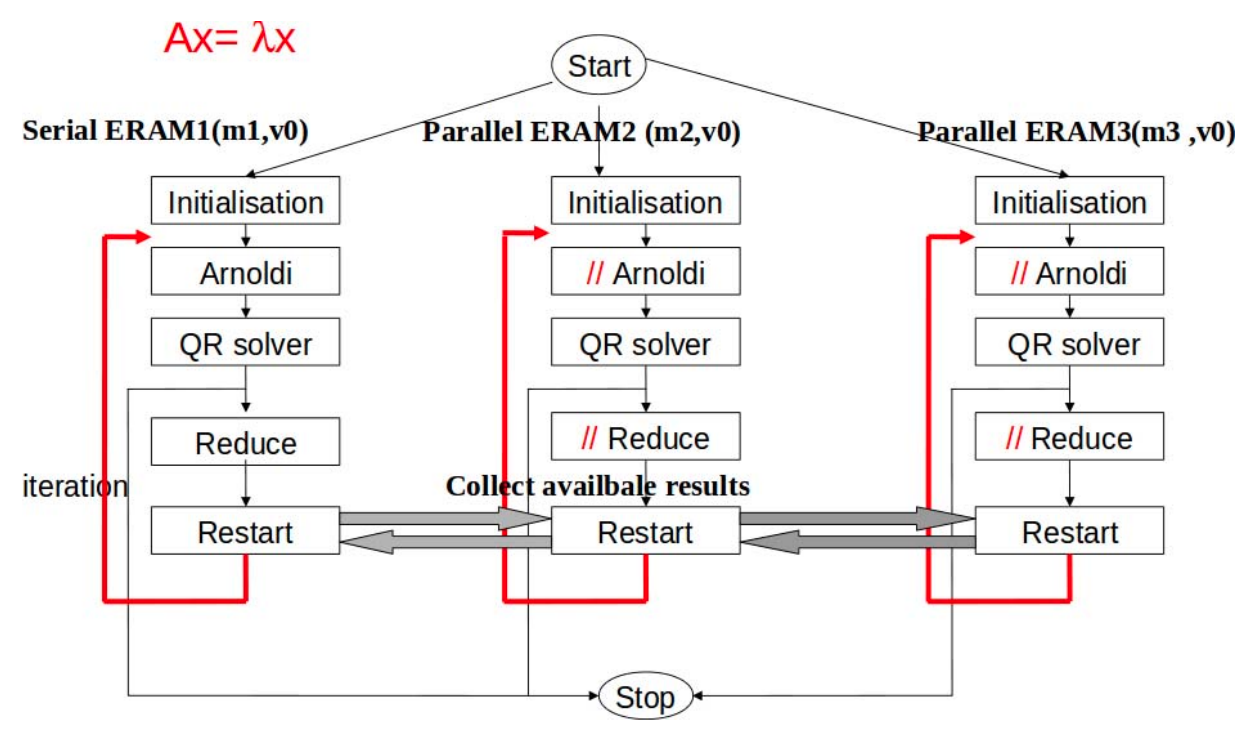
\includegraphics[width=6.3in]{fig/meram.png}
	\caption{An overview of MERAM (\cite{emad2005multiple}).}
	\label{meram}
\end{figure}

\begin{figure}[t]
	\centering
	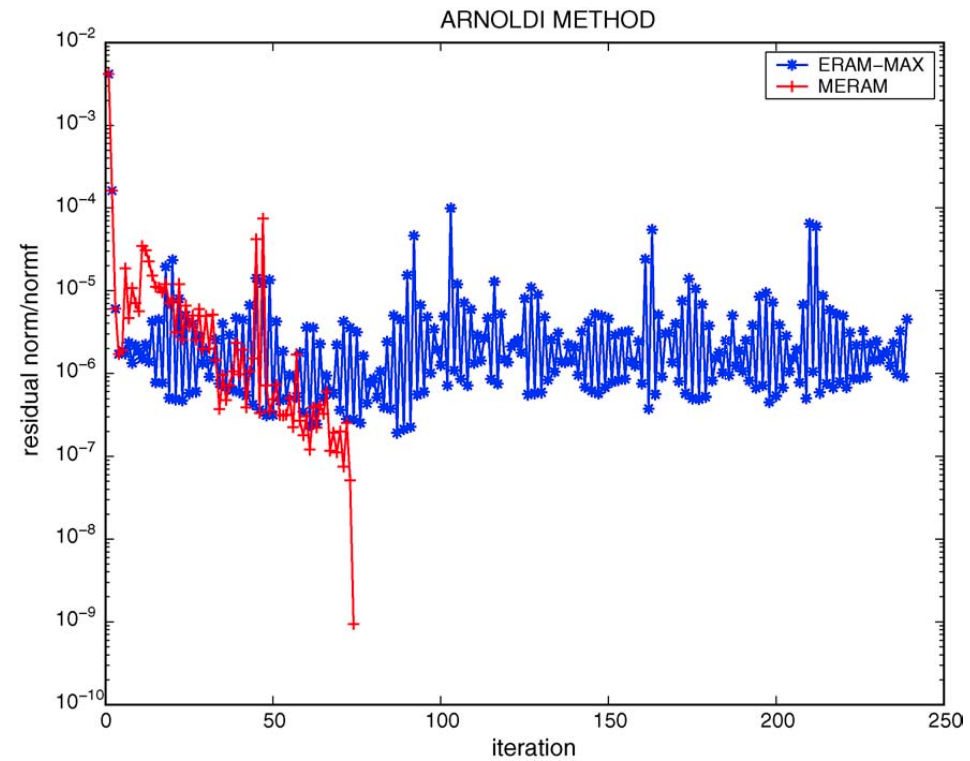
\includegraphics[width=6.2in]{fig/meram_perf.png}
	\caption{An example of MERAM: MERAM(5,7,10) vs. ERAM(10) with af 23560.mtx matrix. MERAM converges in 74 restarts, ERAM does not converge after 240 restarts (\cite{emad2005multiple}).}
	\label{meram-perf}
\end{figure}

\section{Asynchronous Unite and Conquer GMRES/LS-ERAM Method}

In this section, we try to propose a new multi-level parallelism programming paradigm to solve linear systems based on the unite and conquer approach. Thus, firstly Section \ref{Divide of Linear Solvers into Components} divide the preconditioned linear solvers into three components, and then discuss in details the proposed paradigm. In Section \ref{UCGLE}, we give an implementation using this programming model by combining the restarted GMRES with the Least Squares polynomial preconditioner.

\subsection{Divide of Linear Solvers into Components} \label{Divide of Linear Solvers into Components}

As shown in Chapter \ref{Krylov Subspace Methods}, the convergence of linear solvers can be accelerated: 

\begin{enumerate}
	\item by preconditioning matrix;
	\item by the deflation of eigenvalues/eigenvectors;
	\item by the selected polynomials.
\end{enumerate}

For the first type solver, which is preconditioned by selected matrix, it is difficult to divide the linear solver and preconditioning matrix into two independant computing components with asynchronous communications. As shown by Algorithm \ref{alg:rp-gmres} and \ref{alg:lp-gmres} in Chapter \ref{Krylov Subspace Methods}, the preconditioned matrix $M$ should be left or right multiplied with the operator matrix $A$ for each time projection inside the Arnoldi reduction process, which cannot be explicitly seperated. On the other hand, it is much easier to divide explicitly the deflation and the polynomial preconditioned linear solvers into seperate components. 

\begin{figure}[htbp]
	\centering
	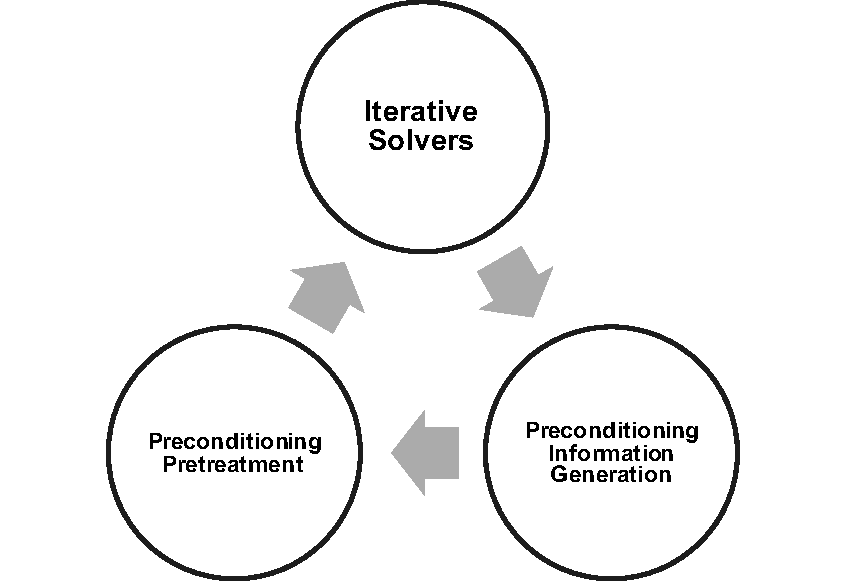
\includegraphics[width=5.2in]{fig/cyclic.pdf}
	\caption{Cyclic Relation of linear solver, eigen-information and preconditioning techniques.}
	\label{fig:cyclic}
\end{figure}

Algorithm \ref{alg:gmres-dr} in \ref{Krylov Subspace Methods} gives an example of deflation preconditioned restarted GMRES. Denote the restart Krylov suspace of this algorithm is $m$, the first cyle of GMRES-DR is the standard Arnoldi reduction which generates $V_{m+1}$ and $\overline{H}_m$. Then the $k$ smallest eigenpairs of $Hm+\beta H_m^{-T}e_me_m^T$ can be approximated, and these eigenpairs are used to construct new $H$ and $V$ with the deflation of these smallest eigenvalues. This solver can be divided into two parts, the first part is a basic restarted GMRES, and the second part is a deflation operations which use the eigenpairs to generate new $H$ and $V$. It is similiar for the hybrid linear solvers preconditioned by the selected polynomial. As shown by Algorithm \ref{alg:hybrid-gmres} which gives a general prototype for the polynomial GMRES. The cycle step of polynomial preconditioned GMRES is also a standard Arnoldi reduction which construct a Hessemberg matrix $H_m$, then selected number of dominant eigenvalues are approximated from $H_m$. The preconditioning step is to refine a polygon from these eigenvalues and get best polynomial $p_k$, $p_k$ is used to generate a new $x_m$ which is used as a new restart vector for the next restarting of GMRES. By analyzing the deflation and polynomial preconditioned linear solvers, it is clear the information used to accelerate are the eigenpairs: for the former, the eigenvalues and eigenvectors of a dense matrix of dimension $m$ related to $H_m$, and then generated new $H$ and $V$; for the latter, the dominant eigenvalues approximated from $H_m$ are used to generate a new restarted vector. In summary, the important information for the preconditioning are the eigenpairs related to $H_m$.  When the solving part and preconditioning part of linear solvers are divided into two computing components, a third computing component should also be provided which is able to generate the eigenpairs. In summary, a new programming paradigm for solving linear systems can be proposed with three kinds of computing components:

\begin{itemize}
	\item \textit{Linear Solver Component} to solve linear systems by standard iterative methods;
	\item \textit{Eigen-Information Component} to generate eigenpairs for the preconditioning process;
	\item \textit{Preconditioning Component} to generate the preconditioned parameters for the Linear Solver Component.
\end{itemize}

Fig. \ref{fig:cyclic} gives a cyclic relation of \textit{Linear Solver Component}, \textit{Eigen-Information Component} and \textit{Preconditioning Component} for the proposed new multi-level programming paradiagm for the deflation and the polynomial preconditioning based on the \textit{Unite and Conquer approach}.

This proposed paradigm is able to accelerate the convergence by the Least Squares polynomial preconditioning, to minimize the number of communications, promote the asynchronisity and reduce the synchronize points by seperation of the preconditioning part and solving part.

This linear solvers based on this novel paradigm are the distributed parallel methods which can profit both shared memory and distributed memory of computational architectures. This new paradigm has two levels of parallelism for distributed memory:

\begin{enumerate}
	\item Coarse Grain/Component level: this paradigm allows the distribution of different numerical components, including the preconditioning part (LS and ERAM) and the solving part (GMRES) on different platforms or processors;
	\item Medium Grain/Intra-component level: the linear solver and Eigen-Information components both deployed in parallel on distributed memory systems;
	\item Fine/Thread level for shared memory: the OpenMP thread level parallelism in CPU, or the accelerator level parallelism if GPUs or other accelerators are available. 
\end{enumerate} 

The reusability of linear solvers based on this new paradigm can be improved, since the preconditioning and solving parts are separated, and the information used for the preconditioning can be saved into local files and reused to solve the subsequent linear systems with the same operator matrix and different RHSs. The fault tolerance of these methods can be also controlled with the implementation of an engine which manage the asynchronous communications of vectors, signals and arrays among different computing components. The exact implementation this manager engine will be presented later in Section \ref{Distributed and Parallel Manager Engine Implementation}.

\subsection{UCGLE Method} \label{UCGLE}

We select the hyrid method preconditioned by the Least Squares polynomial to construct a distributed and parallel linear solver based our new programming model, that is the UCGLE method. In the conventional implementation of this hybrid method, the eigenvalues used to construct the least squares polynomials are computed by the Hessemberg matrix $H_m$ after each time Arnoldi reduction cycle of GMRES. In UCGLE, the linear solver, the approximation of eigenvalues and the construction of least squares polynomials are separated into three different parts. These three computing components work independently with each other and they share the necessary information by the asynchronous communications.

UCGLE method comprises mainly two parts: the first part uses the restarted GMRES method to solve the linear systems; in the second part, it computes a specific number of approximated eigenvalues, and then applies them to the Least Squares method and gets a new preconditioned residual, as a new initial vector for restarted GMRES. 

Figure \ref{fig:worflow} gives the workflow of UCGLE method with three computation components. ERAM Component and GMRES Component are implemented in parallel, and the communication among them is asynchronous. ERAM Component computes a desired number of eigenvalues, and then sends them to LS Component; LS Component uses these received eigenvalues to output a new residual vector, and sends it to GMRES Component; GMRES Component uses this residual as a new restarted initial vector for solving non-Hermitian linear systems.

\begin{figure}[htbp]
	\centering
	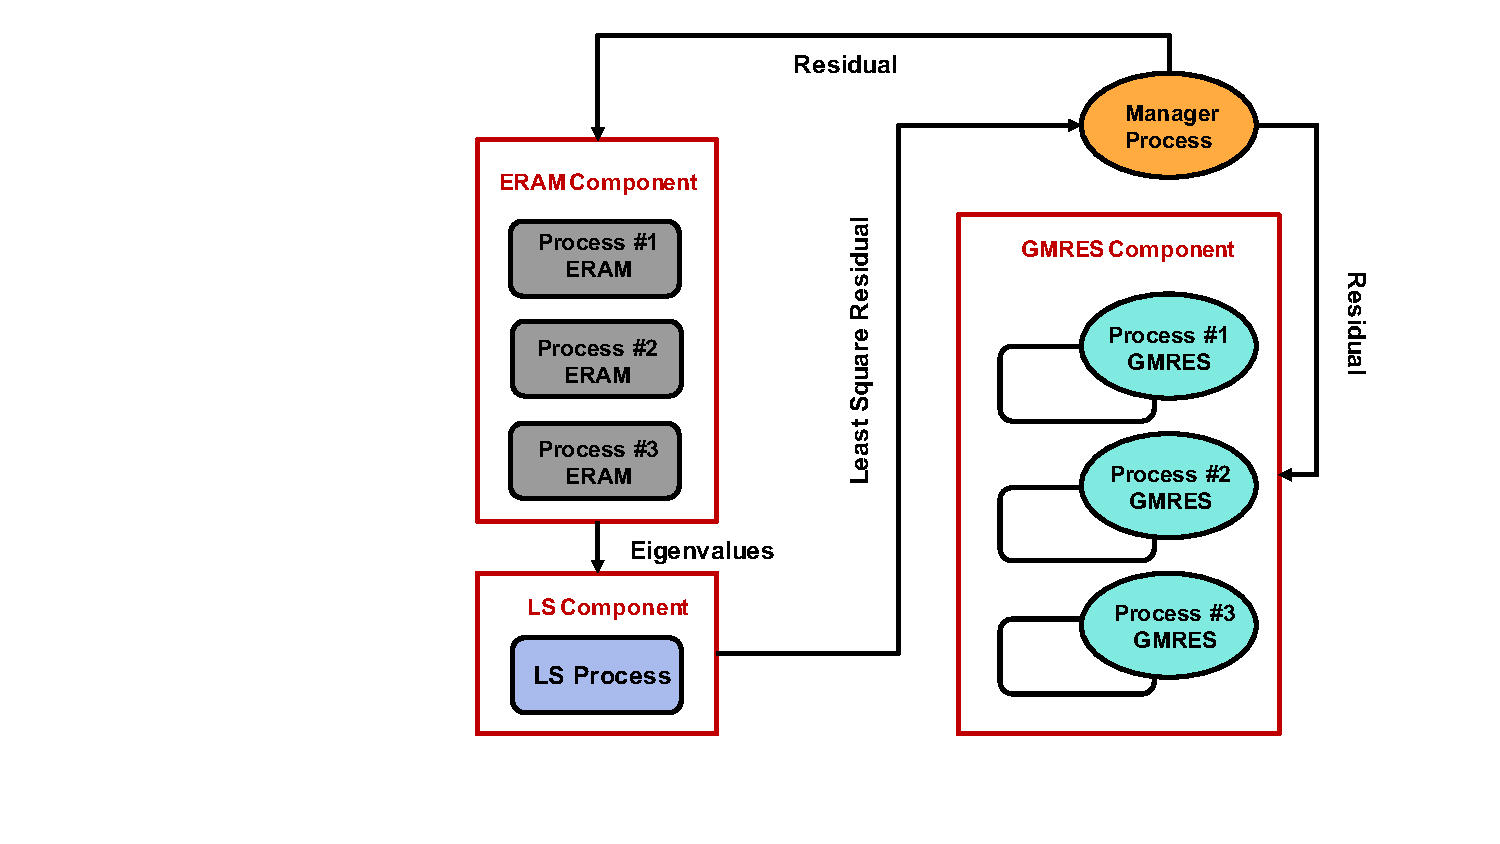
\includegraphics[width=5.2in]{fig/workflow.pdf}
	\caption{Workflow of UCGLE method's three components}
	\label{fig:worflow}
\end{figure}


\section{Distributed and Parallel Implementation}

This section gives the distributed and parallel implementation, including the components, the multi-level parallelism, the manager engine, and the asynchronous communications.
\subsection{Component Implementation}

This section gives the basic implementation and workflow for each component in UCGLE, and Algorithm \ref{alg:gmres/ls-a} gives the implementation of UCGLE in details.

\subsubsection{GMRES Component}

GMRES Component aims to complete the solving a linear system $Ax=b$. It takes as input an operator matrix $A$ and two vectors, $x$ the initial guess vector and $b$ the related RHS. GMRES approximates the solution starting from this initial guess vector until the exact solution is found or if a stopping criterion is met, for example, that the residual norm is below a given threshold (e.g., $||r||_2 \leq 10e^{-8}$). In practice, GMRES are restarted after $m$ steps of iterations in order to reduce the memory requirement. Before each time of restart, GMRES Component check if it receives asynchronously the LS parameters from LS Component. If received, it will provide these parameters to generate a new residual vector and use it as the restart vector, if not, GMRES will be normally restarted. Fig. \ref{gmres-component} gives the workflow of GMRES Component.

GMRES Component loads the parameters $A, m_g, x_0, b, \epsilon_g, L, s_{use}$ to solve the linear systems. At the beginning of the execution, it behaves like the basic GMRES method. When it finishes the $m^{th}$ iteration, it will check if the condition $||b-Ax_m||<\epsilon_g$ is satisfied, if yes, $x_m$ is the solution of linear system $Ax=b$, or GMRES Component will be restarted using $x_m$ as a new initial vector. A parameter $count$ is used to count the times of restart. All these processes are similar to a Restarted GMRES. However, when $count$ is an integer multiple of $L$ (number of GMRES restarts between two times preconditioning of LS), it will check if it has received the parameters $A_d, B_d, \Delta_d, H_d$ from LS Component. If yes, these parameters will be used to construct a preconditioning polynomial $P_d$, which can be used to generate a preconditioned residual $x_d$, then set the initial vector $x_0$ as $x_d$, and restart the basic GMRES, until the exit condition is satisfied.

The GMRES component has the role of solving the linear system.  We reused PETSc's GMRES resolution method and modified it to include sending and receiving data and calculating the new residual. After going through a configuration phase of the numerical method, relating to parameters as important as the size of subspace to be used, as well as the residual standard to be achieved.

\begin{figure}[htbp]
	\centering
	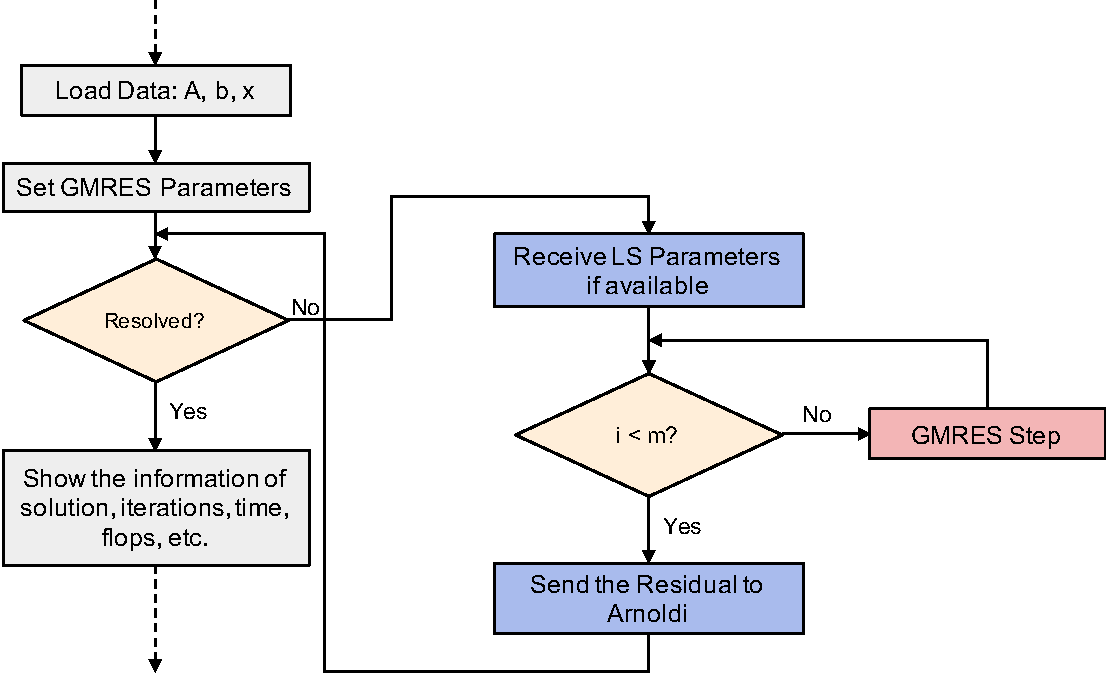
\includegraphics[width=6.2in]{fig/GMRES-component.pdf}
	\caption{GMRES Component.}
	\label{gmres-component}
\end{figure}

\subsubsection{ERAM Component}

\begin{figure}[htbp]
	\centering
	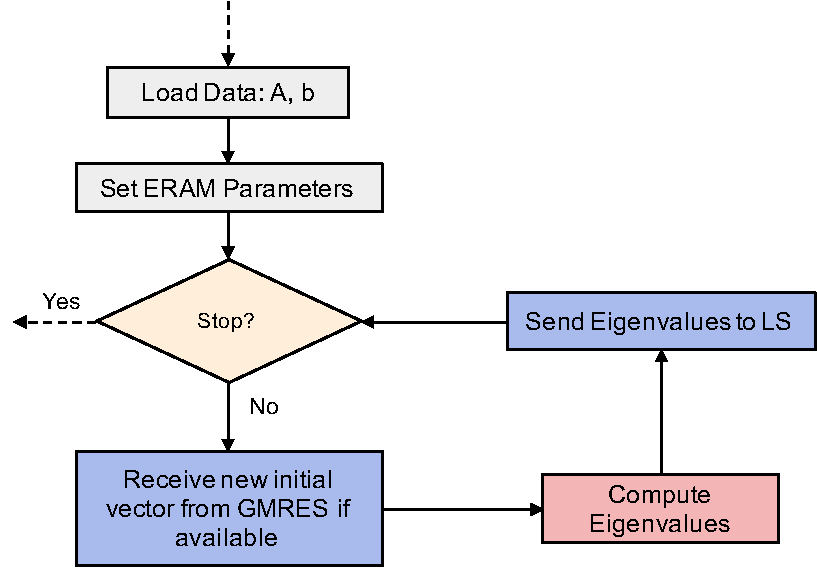
\includegraphics[width=4.8in]{fig/ERAM-component.pdf}
	\caption{ERAM Component.}
	\label{eram-component}
\end{figure}

Fig. \ref{eram-component} gives the workflow of ERAM Component. ERAM Component loads the parameters $m_a, v, r, \epsilon_a$ and the operator matrix $A$, then launches ERAM function. When it receives a new vector $X\_TMP$ from GMRES Component, this vector will be stored in ERAM Component. This vector is updated with the continuous receiving of a new one from GMRES Component. If the $r$ eigenvalues $\Lambda_r$ are approximated by ERAM Component, it will send them to LS Component, at the same time, it is able to save the eigenvalues into the local file.

\subsubsection{LS Component}

Fig. \ref{ls-component} gives the workflow of ERAM Component. LS Component won't start work until it receives the eigenvalues $\Lambda_r$ sent from ERAM Component. Then it will use them to compute the parameters $A_d, B_d, \Delta_d, H_d$, whose dimensions are related to LS parameter $d$, the Least Squares polynomial degree, and send these parameters to GMRES Component.

\begin{figure}[htbp]
	\centering
	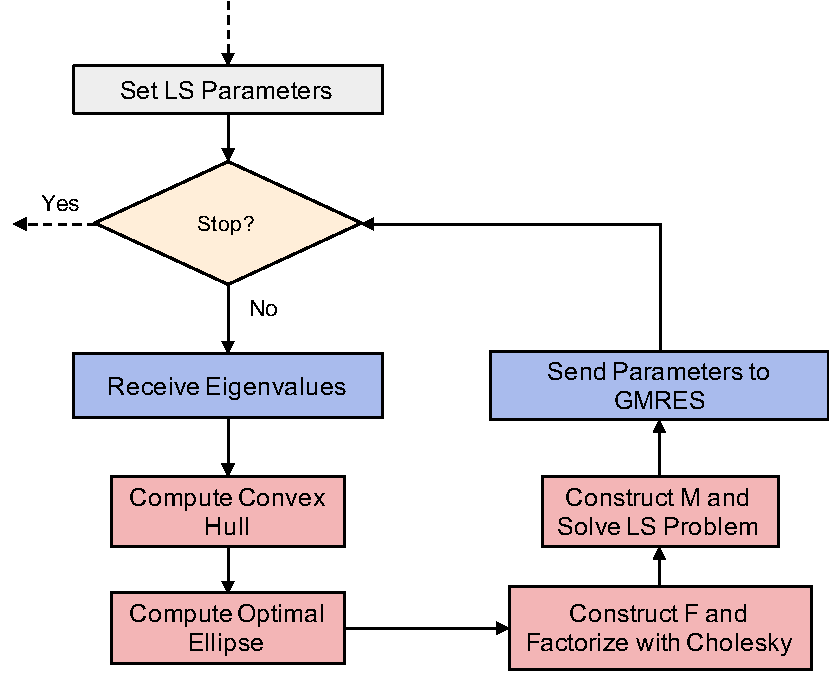
\includegraphics[width=4.8in]{fig/LS-component.pdf}
	\caption{LS Component.}
	\label{ls-component}
\end{figure}

\begin{breakablealgorithm}
	\caption{Implementation of Components}   
	\label{alg:gmres/ls-a}   
	\begin{algorithmic}[1]
		\Function{LOADERAM}{$input$: $A, m_a, \nu, r, \epsilon_a$}
		\While{exit==False}
		\State ERAM($A, r, m_a, \nu,\epsilon_a$, $output$: $\Lambda_r$)
		\State Send ($\Lambda_r$) to LS
		\If{$saveflg==TRUE$} 
		\State write ($\Lambda_r$) to file $eigenvalues.bin$\EndIf
		\If{Recv ($X\_TMP$)} 
		\State update $X\_TMP$\EndIf
		\If{Recv ($exit==TRUE$)} 
		\State Send ($exit$) to LS Component  \State stop \EndIf
		\EndWhile
		\EndFunction
		\Function{LOADLS}{$input$: $A,b, d$}
		\If {Recv($\Lambda_r$)}
		\State LS{($input$: $A,b,d,\Lambda_r$, $output$: $A_d, B_d, \Delta_d, H_d$)}
		\State Send ($A_d, B_d, \Delta_d, H_d$) to GMRES Component
		\EndIf
		\If{Recv ($exit==TRUE$)} 
		\State stop \EndIf
		\EndFunction
		
		\Function {LOADGMRES}{$input$: $A, m_g, x_0, b, \epsilon_g, L, s_{use}$, $output$: $x_m$}
		\State $count=0$
		\State BASICGMRES{($input$: $A, m, x_0,b$, $output$: $x_m$)}
		\State $X\_TMP = x_m$
		\State Send ($X\_TMP$) to ERAM Component
		\If{$||b-Ax_m||<\epsilon_g$}
		\State \Return $x_m$
		\State Send ($exit==TRUE$) to ERAM Component
		\State Stop
		\Else \If{$count \mid L$}
		\If{recv ($A_d, B_d, \Delta_d, H_d$)}
		\State $r_0=f-Ax_0$, $\omega_1 = r_0$ and $x_0=0$
		\For {$k=1,2,\cdots, s_{use}$}
		\For {$i=1, 2, \cdots, d-1$}
		\State $\omega_{i+1}=\frac{1}{\beta_{i+1}}[A\omega_i-\alpha_i\omega_i-\delta_i\omega_{i-1}]$
		\State $x_{i+1}=x_i+\eta_{i+1}\omega_{i+1}$
		\EndFor
		\EndFor
		\State set $x_0=x_d$, and GOTO 1
		\State $count++$
		\EndIf
		\Else
		\State set $x_0=x_m$, and GOTO 1
		\State $count++$
		\EndIf
		\EndIf
		\If{Recv ($exit==TRUE$)} 
		\State stop \EndIf
		\EndFunction
	\end{algorithmic}  
\end{breakablealgorithm}


\subsection{Parameters Analysis} \label{parameter analysis}

UCGLE method is a combination of three different methods, there are a number of parameters, which have impacts on its convergence rate. We summarize these different related ones, and classify them according to their relations with different components.

\begin{enumerate}[]
	\item GMRES Component
	\begin{enumerate}[]
		\item $m_g$: GMRES Krylov Subspace size 
		\item $\epsilon_g$: absolute tolerance for  the GMRES convergence test
		\item $P_g$: GMRES core number
		\item $s_{use}$: number of times that polynomial applied on the residual before taking account into the new eigenvalues
		\item $L$: number of GMRES restarts between two times of LS preconditioning
	\end{enumerate}
	\item ERAM Component
	\begin{enumerate}[]
		\item $m_a$: ERAM Krylov subspace size
		\item $r$: number of eigenvalues required
		\item $\epsilon_a$: tolerance for the ERAM convergence test
		\item $P_a$: ERAM core number
	\end{enumerate}
	\item LS Component
	\begin{enumerate}[]
		\item $d$: Least Squares polynomial degree
	\end{enumerate}
\end{enumerate}

Suppose that the computed convex hull by Least Squares contains eigenvalues $\lambda_1,\cdots, \lambda_m$, the residual given by Least Square polynomial of degree $d-1$ is

\[
r = \sum_{i=1}^{k}\rho_i R_d(\lambda_i)u_i + \sum_{i=m+1}^{n}\rho_i R_d(\lambda_i)u_i
\]

The first part of this residual is minimized by the Least Square polynomial method using the eigenvalues inside convex hull $H_k$, and the second part is large since the related eigenvectors associated with the eigenvalues outside $H_k$. With the number of approximated eigenvalues $d$ increasing, the first part will be much closer to zero and the second part keeps enormous. The next restart process of GMRES can be still accelerated since it restarts with the combination of eigenvectors. The more eigenvalues are known, the more significant acceleration will be. The convergence comparison of UCGLE and classic GMRES is given in Fig. \ref{fig:conv}. The large peaks appear in the UCGLE curve for each time restart. It means that the residual turns to be large, and then will drop down very quickly with the acceleration of LS polynomial method.

\begin{figure}[htbp]
	\centering
	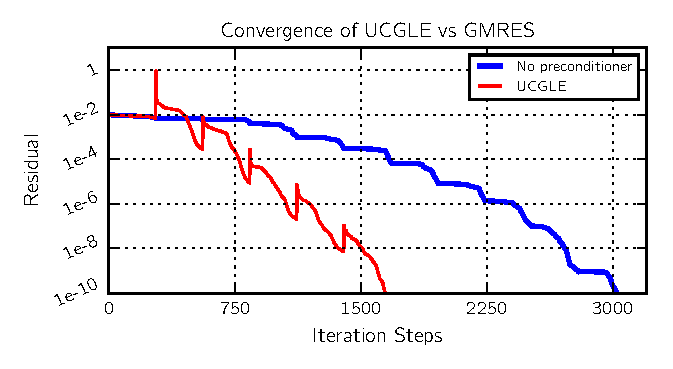
\includegraphics[width=6.2in]{fig/conv.eps}
	\caption{Convergence comparison of UCGLE method vs classic GMRES.}
	\label{fig:conv}
\end{figure}

The Algorithm \ref{alg:gmres/ls-a} shows the implementation of UCGLE's three components and their asynchronous communication in detail. 

\subsection{Distributed and Parallel Manager Engine Implementation}\label{Distributed and Parallel Manager Engine Implementation}

The GMRES method has been implemented by PETSc, and the ERAM method is provided by SLEPc. Additional functions have been added to the GMRES and ERAM provided by PETSc and SLEPc in order to include the sending and receiving functions of different types of data. For the implementation of LS Component, it computes the convex hull and the ellipse encircling the Ritz values of matrix $A$, which allows generating a novel Gram matrix $M$ of selected Chebyshev polynomial basis. This matrix should be factorized into $LL^T$ by the Cholesky algorithm. The Cholesky method is ensured by PETSc as a preconditioner but can be used as a factorization method. The implementation based on these libraries allows the recompilation of the UCGLE codes to adapt to both CPU and GPU architectures. The experimentation of this paper does not consider the OpenMP thread level of parallelism since the implementation of PETSc and SLEPc is not thread-safe due to their complicated data structures. The data structures of PETSc and SLEPc makes it more difficult to partition the data among the threads to prevent conflict and to achieve good performance (\cite{petsc-user-ref}).

\subsubsection{Implementation of the Inter-component Communication Network}

\begin{figure}[t]
	\centering
	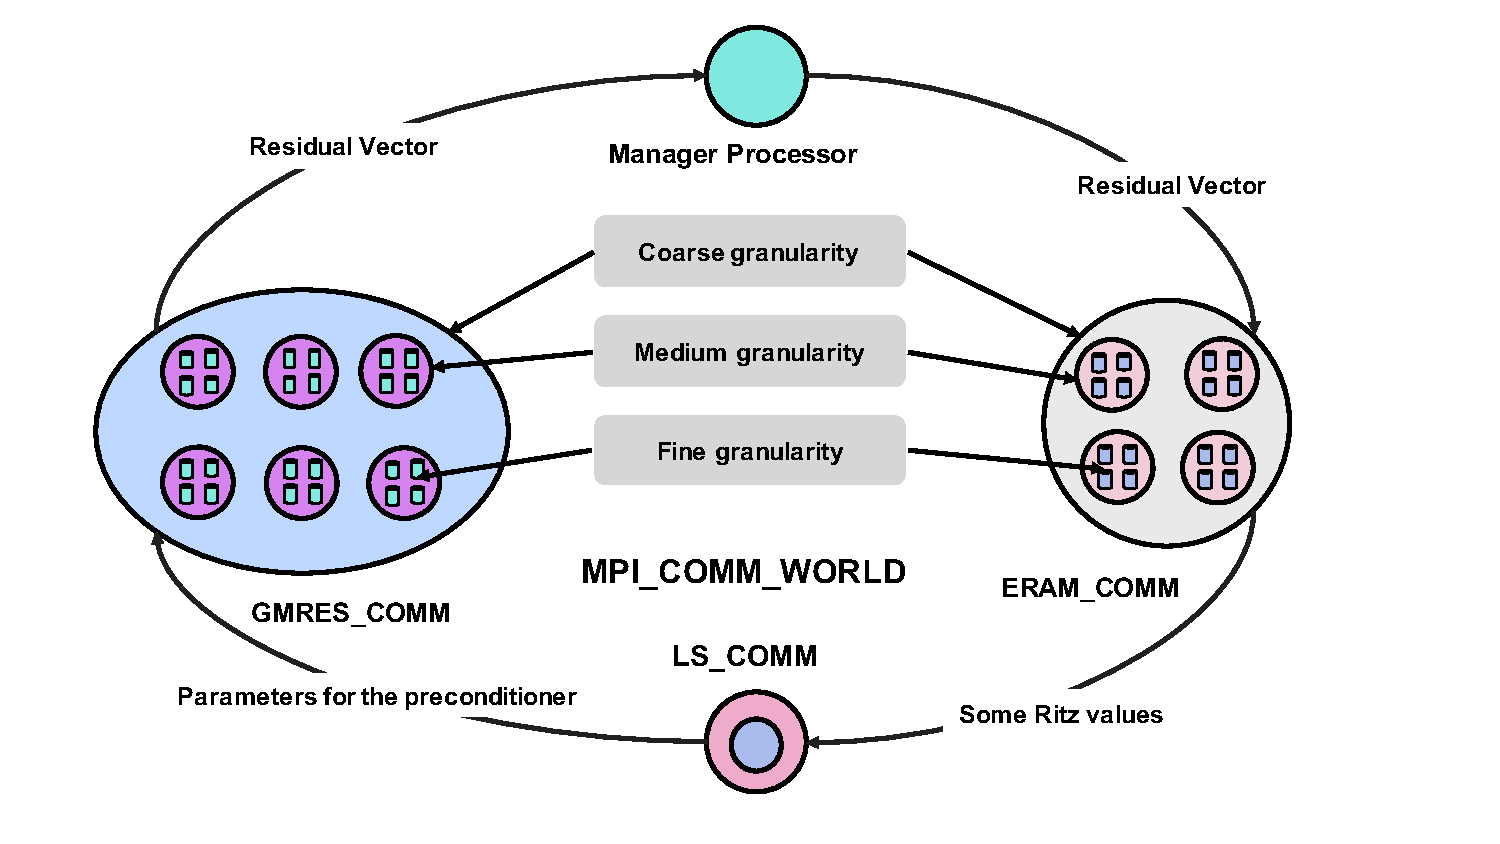
\includegraphics[width=5.2in]{fig/GLSA_MPI.pdf}
	\caption{Communication and different levels parallelism of UCGLE method}
	\label{fig:glsa_mpi}
\end{figure}

From a view of asynchronous communication, the implementation of UCGLE is to establish several communicators inside of $MPI\_COMM\_WORLD$ and their inter-communication. The topology of communication among these groups is a circle shown in Figure \ref{fig:glsa_mpi}. The total number of computing units supplied by the user is thus divided into four groups according to the following distribution: $P_t$ is the total number of processes, then $P_t = P_g + P_a + P_l + P_m$, where $P_g$ is the number of processes assigned to GMRES Component, $P_a$ the number of processes to ERAM component, $P_l$ the number of processes allocated to LS Component and $P_f$ the number of processes allocated to $Manager Process$ proxy. $P_g$ and $P_a$ are greater than or equal to $1$, $P_l$ and $P_m$ are both exactly equal to $1$. LS Component is a serial component because the Least Squares polynomial method cannot be parallelized.

\begin{figure}
	\centering
	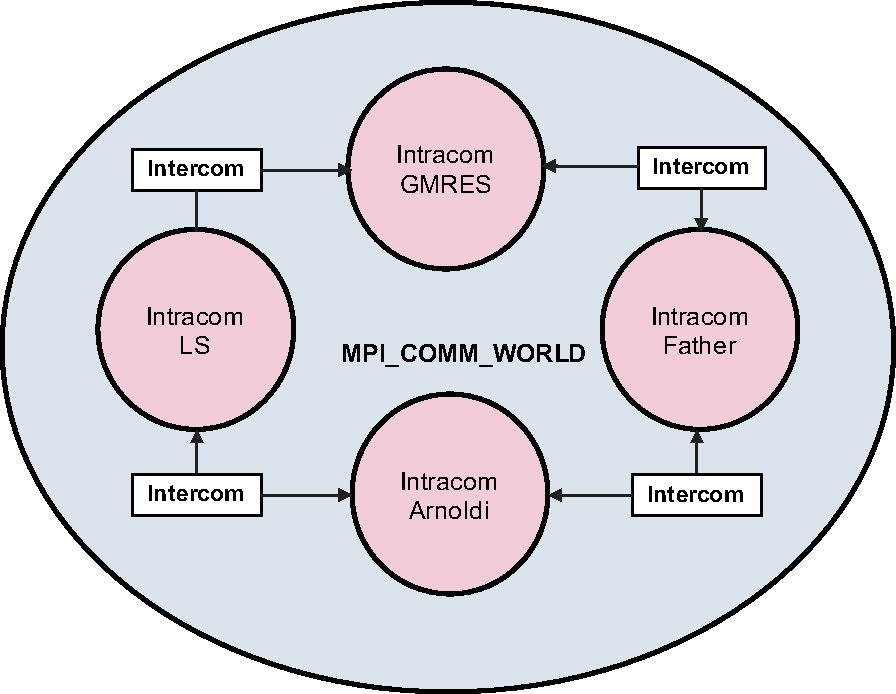
\includegraphics[width=4.2in]{fig/UCGLE_COMM_WORLD.pdf}
	\caption{Creation of Several Intra-Communicators in MPI.}
	\label{fig:ucgle_comm_world}
\end{figure}

$P_t$ is thus divided into several MPI groups according to a color code. The minimum number of processes that our program requires is $4$. We utilize the mechanism of MPI standard to support the communication of our application fully. The communication layer that does not depend on the application, this allows the replacement and scalability of various components provided.

\subsubsection{Asynchronous Communication Mechanism}

As shown in Figure \ref{fig:glsa_mpi}, UCGLE has three levels of parallelism which is suitable for the modern supercomputers. In fact, the main characteristic of UCGLE method is its asynchronous communication. But the synchronous communication takes place inside of GMRES and ERAM components. Distributed and parallel communication involves different types of exchange data, such as vectors, scalar tables, and signals among different components. When the data are sent and received in a distributed way, it is essential to ensure the consistency of data. In our case, we choose to introduce an intermediate node as a proxy to carry out only several types of exchanges and thus facilitate the implementation of asynchronous communication. This proxy is called \textit{Manager Process} as in Figure \ref{fig:glsa_mpi}. One process can fulfill all the data exchanges.

\begin{figure}[t]
	\centering
	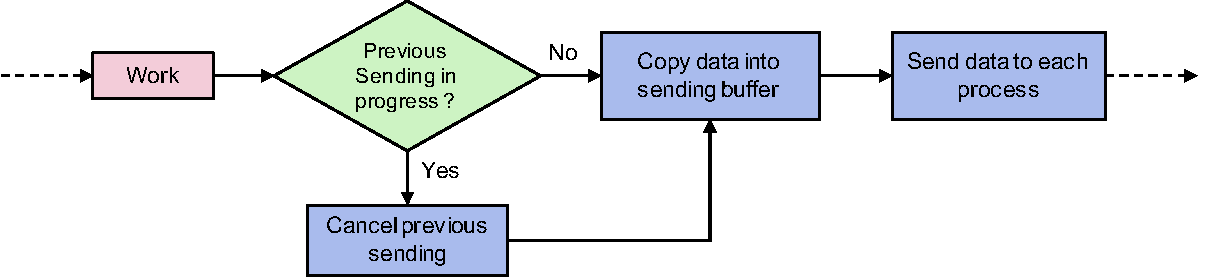
\includegraphics[width=6.2in]{fig/send.pdf}
	\caption{Data Sending Scheme from one group of process to the other.}
	\label{fig:send}
\end{figure}

Asynchronous communication allows each computation component to conduct independently the work assigned to it without waiting for the input data. The asynchronous data sending and receiving operations are implemented by the non-blocking communication of Message Passing Interface (MPI). Sending takes place after the sender has completed the task assigned to it. Before any prior shipment, the component checks whether several transactions are now on the way. If yes, this task will be canceled to avoid the competition of different types of sending tasks. Sent data are copied into a buffer to prevent them from being modified while sending. For the asynchronous data receiving, before starting this task, the component will check if data is expected to be received. Once the receiving buffer is allocated, the component performs the receiving of data while respecting the distribution of data globally according to the rank of sending processes. It is also essential to validate the consistency of receiving data before any use of them by the tasks assigned to the components.


\textbf{Asynchronous Sending:} The sending operation, as we described, will start by verifying if the previous sending operations are pending or not. If some operations are not finished, they are canceled so as not to be in a state where several shipments with different data are in competition. In the practical implementation, we use the MPI\_Request to track the state of an asynchronous request. Once the verification is validated, then the data to be sent will be copied to a buffer to prevent them overwritten by other work operations. Then, this data is sent to the different nodes of the other components, respecting the distribution negotiated during the initialization of the communications via the standard asynchronous sending function MPI\_Isend.

This last function is asynchronous in the sense that the data sent with this function will only be effective when the recipient (s) decide to receive them. In practice, it may be interesting to know that this is not entirely true. Indeed, the actual sending of data only occurs when the receiver or receivers are available, but also during a subsequent call to the MPI library whatever it is. Thus it may be that the sending cannot be done because the communicating nodes do not find the time to communicate. 

\begin{figure}[t]
	\centering
	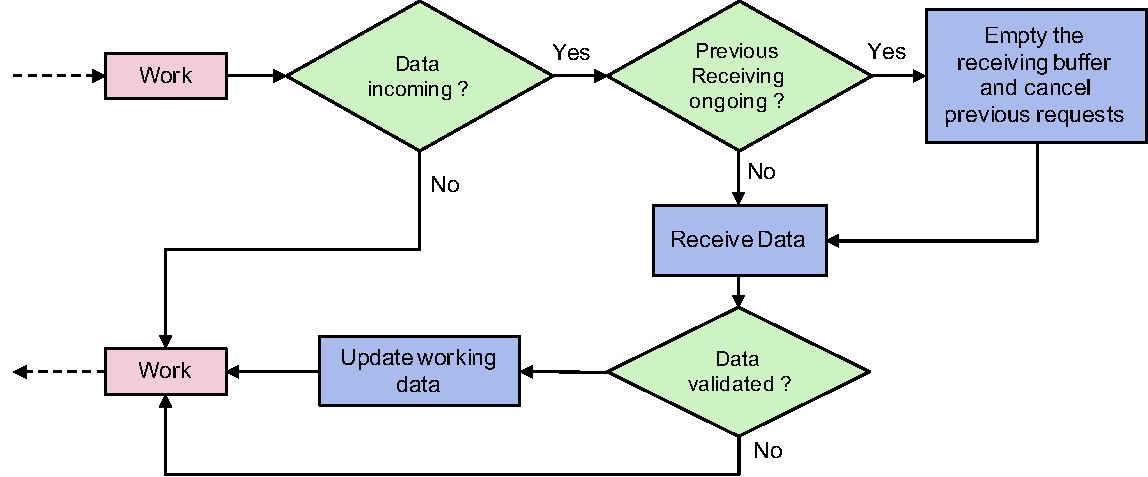
\includegraphics[width=6.2in]{fig/recv.pdf}
	\caption{Data Receiving Scheme from one group of process to the other.}
	\label{fig:recv}
\end{figure}

\textbf{Asynchronous Receiving:} In the context of send-and-receive communication mechanisms, the sending operation is often the most difficult to implement because it requires a synchronization point. As far as we are concerned, we have hidden this synchronization point thanks to an input verification step. Indeed, we have chosen to implement a test function before proceeding with asynchronous reception instead of going through a purely asynchronous reception function. The data input test is done via the MPI\_Iprobe function and the MPI\_Recv reception. The latter is blocking or synchronous, that is, once called the computation node will wait for data to be received before returning to the calling function. 

At first glance, it would seem wiser to go through the non-blocking reception function MPI\_Irecv, but in practice, this function requires to know in advance the size of the data that will be received, which is not the case in the case where our components exchange tables of scalars. Indeed, the component Arnoldi goes throughout its task, calculate more and more eigenvalues, more and more precise. In advance, it is not possible to know the number of eigenvalues that will be obtained, in fact, impossible to predict the size of the input buffer. Also, we made a choice to work with a dynamic reception buffer. In our implementation, this one is allocated thanks to the information provided by the operation MPI\_Get\_count using structure MPI\_Status filled in by the function MPI\_Iprobe.

Also, apart from this difference, our reception mechanism is fundamentally similar to the MPI\_Irecv function in that it only receives data if it is available. In our case we also do not receive data if they are not available, the component to continue its task in case they were not. 

In addition to having reimplemented MPI's asynchronous receive mechanism, we integrated a mechanism for checking the consistency of the received data. In order to allow different independent groups of compute nodes (our components), we have used the tools that are the intracommunicators and inter-communicators MPI (see explanations in 5.2.3.1). The problem of this type of implementation (at the same time there is no other possible, at least without falling into the experimental unstable) is that it does not allow collective communications between the different nodes of two communicating groups. In fact, the communications between groups of nodes (or components) pass through the intercommunication that only allow collective communications between those between the master of a group and the set of nodes of the other. This is therefore quite limiting when the goal (ours) is to carry out entirely collective communications, that is to say to allow all the nodes of a group to communicate with all the nodes of another group. This is what we have completed through our implementation of the sending and receiving mechanisms. The real problem is as to the coherence of the received data.

Indeed, even if we go through the proxy to facilitate communication control, data consistency must be checked before any prior use. For example, take the case of a vector. If a vector is partially received, it can not be used, and if it was the case, we could witness a disaster from a numerical point of view. Also, to avoid this kind of pitfall, we have integrated a validation mechanism that will check that the received data are consistent before they are used. The consistency check is conveniently performed by comparing the total size of the data received by each component node against the size of the data to be received at all. If this is consistent, then the reception buffer data is placed in the working memory of each node of the receiving component.

\subsubsection{Implementation for Hetergeneous Platforms with Multi-GPU}

\textcolor{red}{TO DO}

\section{Experiment and Evaluation}

\subsection{Hardware Platforms}

We test its convergence acceleration, fault tolerance and scalability on the large-scale platforms. UCGLE method has been installed on the supercomputer \textit{Tianhe-2}, which is installed at the National Super Computer Center in Guangzhou of China. It is a heterogeneous system made of Intel Xeon CPUs and Intel Knights Corner (KNC), with 16000 compute nodes in total. Each node composes 2 Intel Ivy Bridge 12 cores @ 2.2 GHz. In this article, we do not test UCGLE with KNC on \textit{Tianhe-2} since PETSc do not support it with good performance.

\subsection{Parameters Evaluation}

\subsubsection{Test Parameters Setup}

\begin{itemize}
	\item \textbf{Krylov subspace size for GMRES }
	\item \textbf{LS applied times: }
	\item \textbf{LS Frequence:}
\end{itemize}

\begin{itemize}
	\item \textbf{Number of eigenvalues: }
\end{itemize}

\begin{itemize}
	\item \textbf{LS polynomial degree: }
\end{itemize}

\subsubsection{Test Matrix Suite: }

\textbf{Matrices from Matrix Market Collections: }
\begin{table}[htbp]
	\renewcommand{\arraystretch}{1.4}
	\small	
	\caption{Test Matrix from Matrix Market Collection.}
	\label{testmatrixforparameters}
	\centering
	\begin{tabular}{c|c|c|c}
		\toprule
		Matrix  & Size & $s$ NNZ & $s$ Domain\\
		\midrule
		utm300  & $300$ & $3155$ &$\mathbb{R}$ \\
		utm1700b & $1700$ & $21509$  & $\mathbb{R}$ \\
		pde2961 & $2961$ & $14585$& $\mathbb{R}$ \\
		young4c & $841$ & $4089$& $\mathbb{C}$ \\
		\bottomrule
	\end{tabular}
\end{table}

\textbf{Matrices generated by SMG2S: }

\subsubsection{Experiments}

In order to highlight the impacts of different parameters inside UCGLE, we conducted several sets of experiments, which varies one parameter mentioned above, and keeps the other parameters fixed. In this section, we will present the results of these experiments, and then analysis the effect of each parameter on the preconditioning, thus the acceleration of convergence. We study the parameters including the Krylov subspace size of GMRES $m_g$, the times of LS preconditioning applied on the GMRES $lsa$, the frequence of LS precondtioning applied $freq$, the number of eigenvalues approximated by ERAM Component $n_{eigen}$, and the degree of LS polynomial $l$.

\textbf{Krylov subspace size: }

The parameter $m_g$, which means the restarted subspace size of GMRES, has important influence on the convergence of UCGLE.  This effect is similiar with the case on the conventional GMRES without preconditioning. For the experiments of UCGLE, we vary $m_g$ from $50$ to $180$, and keep $l=10$, $lsa=10$, $freq=10$. Moverover, we evaluate also the classic GMRES with $m_g$ to be $100$ and $150$. The results are given in Fig. \ref{fig:krylovsubspace}. First of all, we can conclude that in the case that $m_g$ is too small (see UCGLE($m_g=50$) in  Fig. \ref{fig:krylovsubspace}), even the LS preconditioning is applied, the convergence can not be achieved. With the augmentation of $m_g$, UCGLE is able to converge with less iteration steps. Secondly, with the preconditioning of LS polynomial, UCGLE can converge with $m_g=100$, but the classic GMRES cannot converge with the same value of this parameter.

In conclusion, the Krylov subspace size of GMRES Component is a very important parameter of UCGLE. If this parameter is too small, it is difficult to get the convergence even with the LS polynomial preconditioning. It is not practical to use very large $m_g$ since the limitation of memory. Thus, it is essential to determine a good value of $m_g$ which is able to able to accelerate the convergence by LS polynomial.

\begin{figure}[htbp]
	\centering
	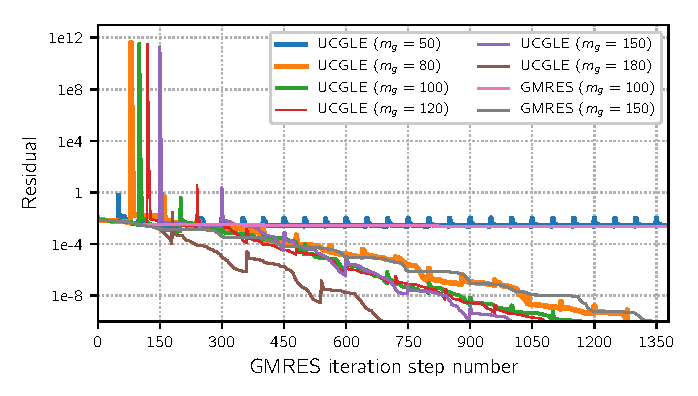
\includegraphics[width=6.2in]{fig/conv_ksp_gmres.eps}
	\caption{Evaluation of GMRES subspace size $m_g$ varying from $50$ to $180$. $l=10$, $lsa=10$, $freq=10$.}
	\label{fig:krylovsubspace}
\end{figure}


\textbf{LS polynomial degree: }

The parameter LS applied times $lsa$ means the number of times the LS parameters will be applied to the temporary solution of GMRES Component before its restart after $m_g$ iterations. In the experiments, $lsa$ ranges from $1$ to $25$, and the parameters $m_g$, $l$, and $freq$ are respectively fixed as $100$, $10$ and $1$. Fig. \ref{fig:Lsappliedtime} shows the convergence curves of all the tests. Firstly, it is obvious that $lsa$ has the effect on the peaks for each time LS preconditioning. The greater it is, the bigger the peak will be. As talked in Section \ref{parameter analysis}, these peaks means the Euclidien norm of restart vector produced by LS polynomial. By comparing the curves in  the Fig. \ref{fig:Lsappliedtime}, we can conclude that the augmentation of $lsa$ wil accelerate the convergence of UCGLE. But, this parameter cannot be too large, this might lead to a too large norm of the residual of the restarted vector generated by LS polynomial preconditioning processus, and finally damage the convergence.

To conclude on the effect of this parameter, it is necessary to select the best value with considering the selection of the parameter of LS polynomial power $l$. In fact, the two parameters seem particularly intricate together and the choice of one will depend on the choice of the other. In the pratical implementation, this parameter implies a series of SpMV and AXPY operations in parallel. The larger $l$ is, the more operations will be executed, thus the more time will be occupied. The good selection of this parameter should make a balance between the reduction of iteration steps of GMRES components and additional time caused by these SpMV and AXPY operations.

\begin{figure}[htbp]
	\centering
	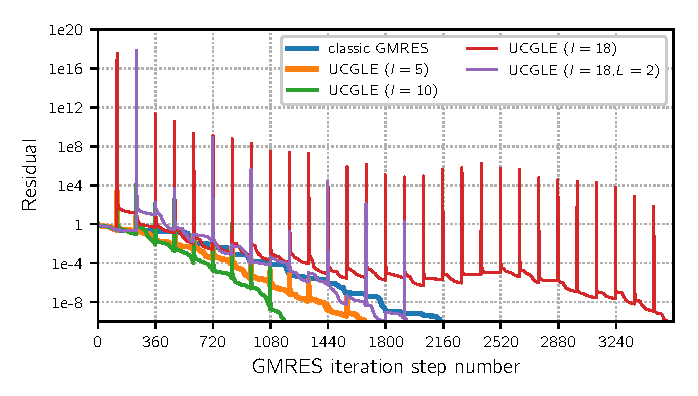
\includegraphics[width=6.2in]{fig/conv2.eps}
	\caption{Convergence comparison of UCGLE method vs classic GMRES.}
	\label{fig:lsdegree}
\end{figure}

\textbf{LS applied times: }

The parameter LS applied times $lsa$ means the number of times the LS parameters will be applied to the temporary solution of GMRES Component before its restart after $m_g$ iterations. In the experiments, $lsa$ ranges from $1$ to $25$, and the parameters $m_g$, $l$, and $freq$ are respectively fixed as $100$, $10$ and $1$. Fig. \ref{fig:Lsappliedtime} shows the convergence curves of all the tests. Firstly, it is obvious that $lsa$ has the effect on the peaks for each time LS preconditioning. The greater it is, the bigger the peak will be. As talked in Section \ref{parameter analysis}, these peaks means the Euclidien norm of restart vector produced by LS polynomial. By comparing the curves in  the Fig. \ref{fig:Lsappliedtime}, we can conclude that the augmentation of $lsa$ wil accelerate the convergence of UCGLE. But, this parameter cannot be too large, this might lead to a too large norm of the residual of the restarted vector generated by LS polynomial preconditioning processus, and finally damage the convergence.

To conclude on the effect of this parameter, it is necessary to select the best value with considering the selection of the parameter of LS polynomial power $l$. In fact, the two parameters seem particularly intricate together and the choice of one will depend on the choice of the other. In the pratical implementation, this parameter implies a series of SpMV and AXPY operations in parallel. The larger $l$ is, the more operations will be executed, thus the more time will be occupied. The good selection of this parameter should make a balance between the reduction of iteration steps of GMRES components and additional time caused by these SpMV and AXPY operations.

\begin{figure}[htbp]
	\centering
	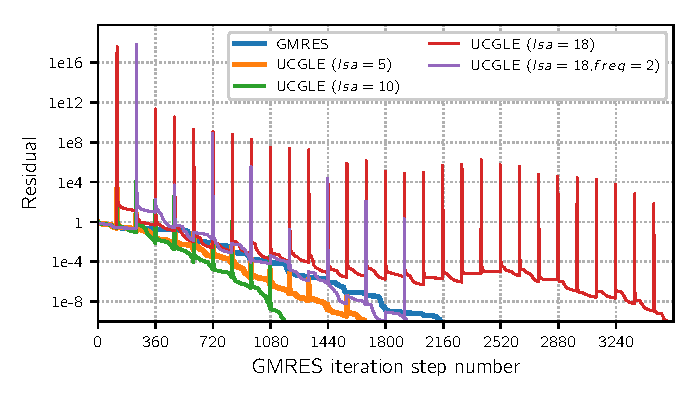
\includegraphics[width=6.2in]{fig/conv_lsappied.eps}
	\caption{Evaluation of LS applied times $lsa$ varying from $1$ to $25$, and $m_g=100$, $l=10$, $freq=1$. }
	\label{fig:Lsappliedtime}
\end{figure}


\textbf{LS Frequence:}

The preconditioning latency represents the number of restarts between which a GMRES preconditioning phase will take place, ie the application of the polynomial to the temporary solution of the resolution method. Also, we noticed previously that after each preconditioning phase corresponded the appearance of a peak of convergence before each acceleration of this one.

In order to characterize the latency parameter (identified by cof in Figures 5.20, 5.21 and 5.22) we conducted a series of tests. These tests were designed to evaluate the number of completed iterations for different latencies, for different subspace sizes.

The results we obtained allowed us to observe several things. The first is that the subspace size is decisive in the preconditioning of the problem. Indeed, if the subspace size is too small then it appears that the preconditioning is not interesting to use. Thus, in the case of too small subspace sizes, preconditioning degrades convergence.  Moreover, in the case where the subspace size GMRES is sufficiently large, then the latency parameter loses its importance. This is something we observe in figure 5.22 where the curves corresponding to the resolutions without preconditioning tend to aggregate together.

Ultimately the latency parameter must be chosen to allow sufficient consideration of the preconditioning in the successive cycles at this stage while not being too important so that the convergence can continue to benefit from its effect at a satisfactory pace.

\begin{figure}[htbp]
	\centering
	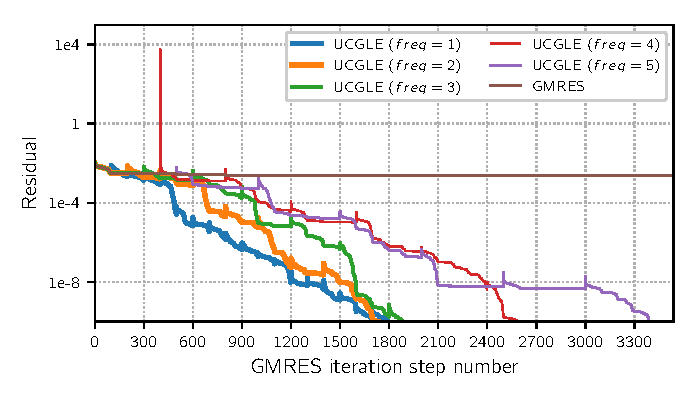
\includegraphics[width=6.2in]{fig/conv_lsfreq.eps}
	\caption{Evaluation of LS applied times $freq$.}
	\label{fig:Lsfreq}
\end{figure}


\textbf{Number of eigenvalues: }

The parameter $m_g$, which means the restarted subspace size of GMRES, has important influence on the convergence of UCGLE.  This effect is similiar with the case on the conventional GMRES without preconditioning. For the experiments of UCGLE, we vary $m_g$ from $50$ to $180$, and keep $l=10$, $lsa=10$, $freq=10$. Moverover, we evaluate also the classic GMRES with $m_g$ to be $100$ and $150$. The results are given in Fig. \ref{fig:krylovsubspace}. First of all, we can conclude that in the case that $m_g$ is too small (see UCGLE($m_g=50$) in  Fig. \ref{fig:krylovsubspace}), even the LS preconditioning is applied, the convergence can not be achieved. With the augmentation of $m_g$, UCGLE is able to converge with less iteration steps. Secondly, with the preconditioning of LS polynomial, UCGLE can converge with $m_g=100$, but the classic GMRES cannot converge with the same value of this parameter.
The subspace size is a parameter that can be considered as one of the most important in the case of the hybrid method. Too small it does not allow to take into account the preconditioning, too big, it will probably not allow it. Influencing both the effect of preconditioning and the convergence of the method, the subspace size must be dimensioned properly to allow the method to converge and precondition to cause the acceleration of the resolution.

\begin{figure}[htbp]
	\centering
	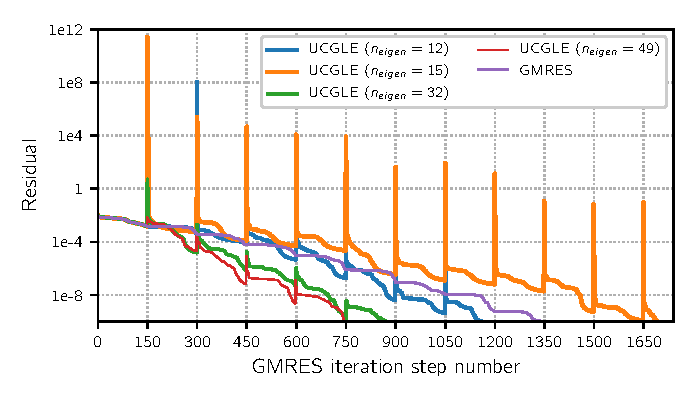
\includegraphics[width=6.2in]{fig/conv_eigenvalues.eps}
	\caption{Evaluation of eigenvalue number $n_{eigen}$.}
	\label{fig:vals}
\end{figure}

\subsection{Convergence Evaluation}

We have selected four test matrices generated by SMG2S using different given spectra to evaluate the convergence speedup of UCGLE method. The first test matrix $MEG1$ and the second matrix $MEG2$ are all generated randomly inside an annulus with different scale which is symmetric to the real axis in complex plane. The size of $MEG1$ is \num[round-precision=2,round-mode=figures]{18000000}, and the size of $MEG2$ is \num[round-precision=4,round-mode=figures]{10240000}. The convergence of UCGLE is compared with 1) the restarted GMRES without preconditioning, 2) restarted GMRES with Jacobi preconditioner, 3) restarted GMRES with SOR preconditioner. We select the Jacobi and SOR preconditioners for the experimentations because they are well implemented in parallel by PETSc. The GMRES restarted parameter for $MEG1$, $MEG2$, $MEG3$ and $MEG4$ are respectively 250, 280, 30 and 40.

\begin{figure}[htbp]
	\centering
	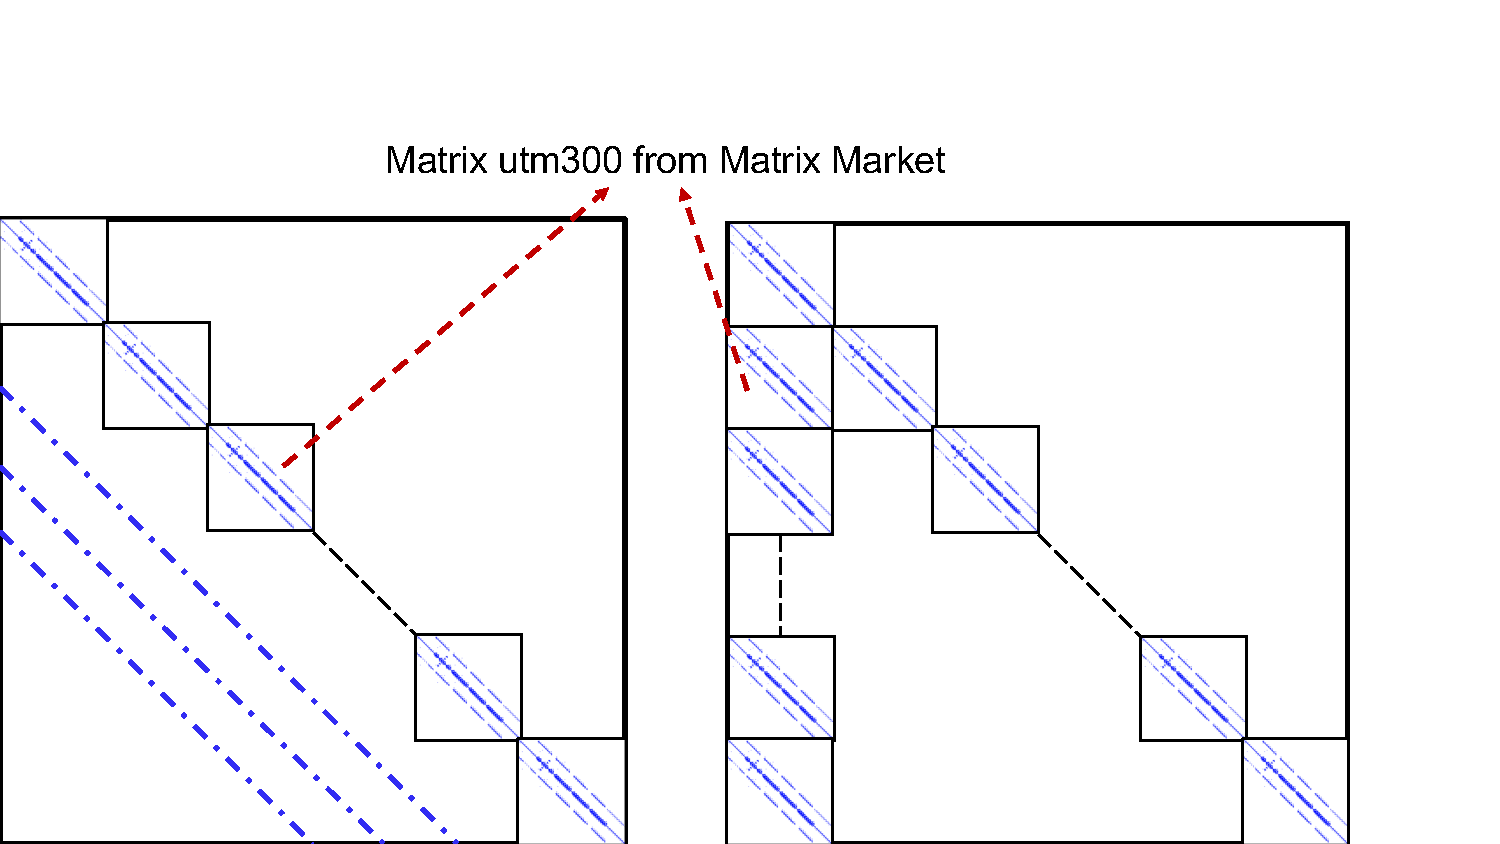
\includegraphics[width=4.2in]{fig/matrix_generator.pdf}
	\caption{Two strategies of large and sparse matrix generator by a original matrix utm300 of Matrix Market.}
	\label{fig:matrix}
\end{figure}


\begin{table}[!t]
	\renewcommand{\arraystretch}{1.2}
	\caption{Test matrices information}
	\label{matget}
	\centering
	\begin{tabular}{|c|c|c|c|}
		\hline
		Matrix Name& n & nnz & Matrix Type\\
		\hline
		$matLine$  & \num[round-precision=2,round-mode=figures]{18000000} & \num[round-precision=2,round-mode=figures]{28823000} & non-Symmetric\\
		\hline
		$matBlock$  & \num[round-precision=2,round-mode=figures]{18000000} & \num[round-precision=2,round-mode=figures]{192160000} & non-Symmetric\\
		\hline
		$MEG1$ & \num[round-precision=4,round-mode=figures]{10240000} & \num[round-mode = places, scientific-notation = fixed, fixed-exponent = 9,round-precision = 2]{7270272000} & non-Hermitian\\
		\hline
		$MEG2$ & \num[round-precision=2,round-mode=figures]{5120000} & \num[round-mode = places, scientific-notation = fixed, fixed-exponent = 9,round-precision = 2]{3635136000} & non-Hermitian\\
		\hline
	\end{tabular}
\end{table}


Fig \ref{fig:conv1}, Fig \ref{fig:conv2}, Fig \ref{fig:conv3} and Fig \ref{fig:conv4} present respectively the convergence experiments of $MEG1$, $MEG2$, $MEG1$ and $MEG2$. The numbers of iteration steos for convergence are given in Table \ref{iterations}. Obviously, UCGLE method has spectacular acceleration on the convergence for both of them over the conventional preconditioners. It has almost two times of acceleration than the SOR preconditioned GMRES. The SOR preconditioned GMRES is already better than the Jacobi preconditioned GMRES and GMRES without preconditioning for the test matrices.

\begin{figure}[htbp]
	\centering
	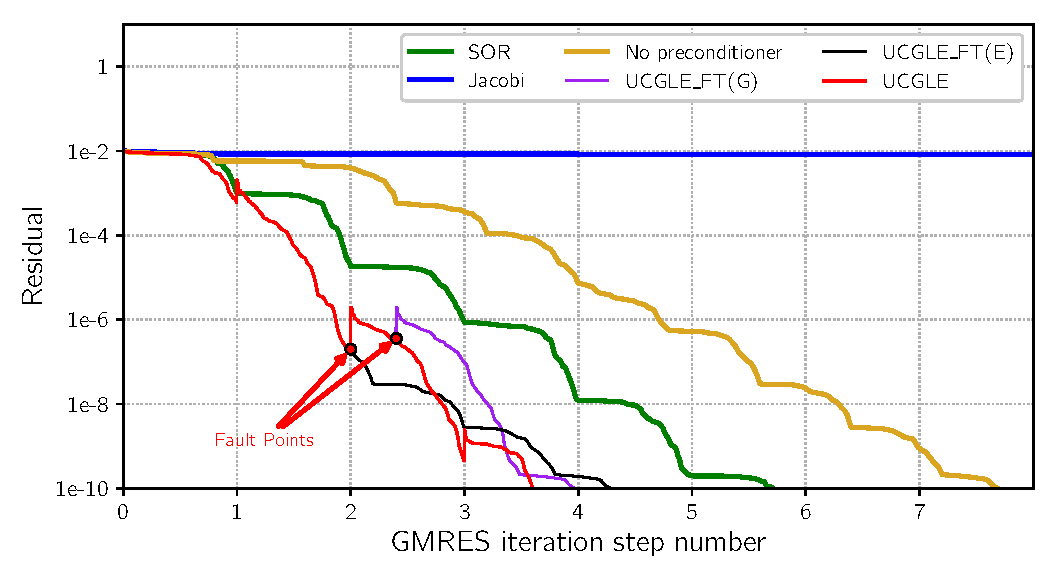
\includegraphics[width=6.2in]{fig/convergence1.eps}
	\caption{$MEG1$: convergence comparison of UCGLE method vs conventional GMRES}
	\label{fig:conv1}
\end{figure}

\begin{figure}[htbp]
	\centering
	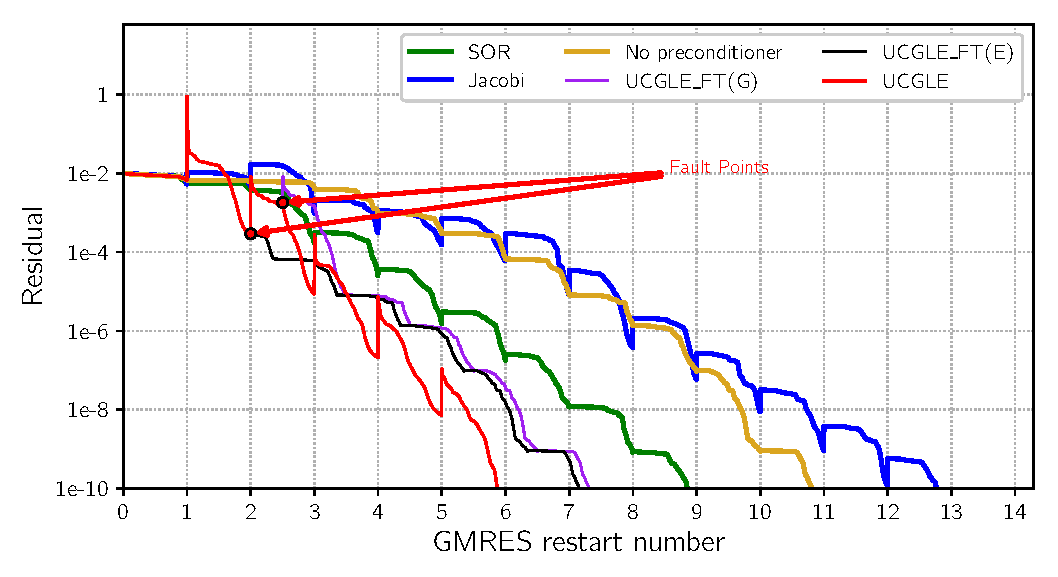
\includegraphics[width=6.2in]{fig/convergence2.eps}
	\caption{$MEG2$: convergence comparison of UCGLE method vs conventional GMRES}
	\label{fig:conv2}
\end{figure}

\begin{figure}[htbp]
	\centering
	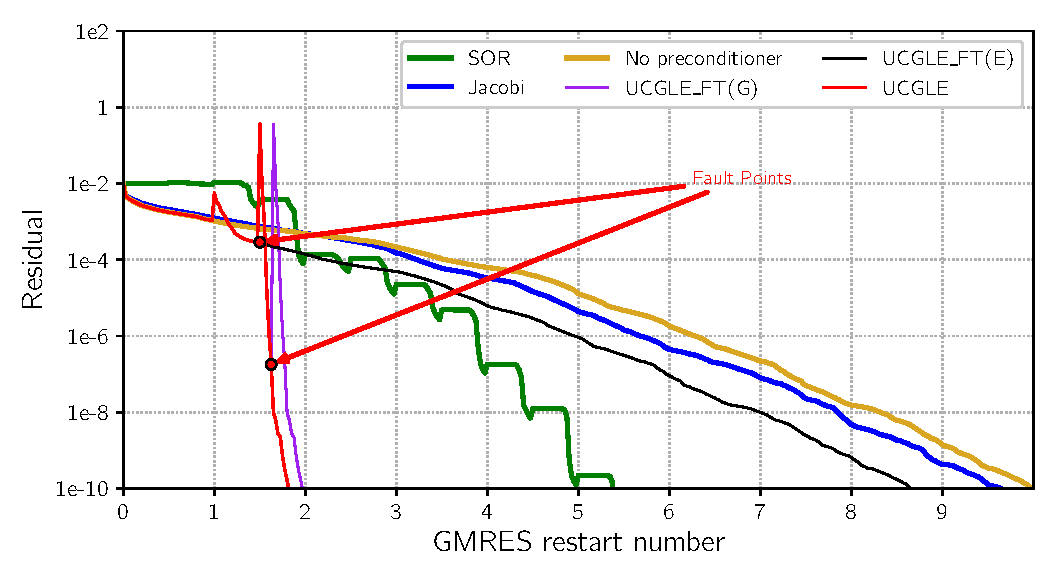
\includegraphics[width=6.2in]{fig/convergence3.eps}
	\caption{$MEG3$: convergence comparison of UCGLE method vs conventional GMRES}
	\label{fig:conv3}
\end{figure}

\begin{figure}[htbp]
	\centering
	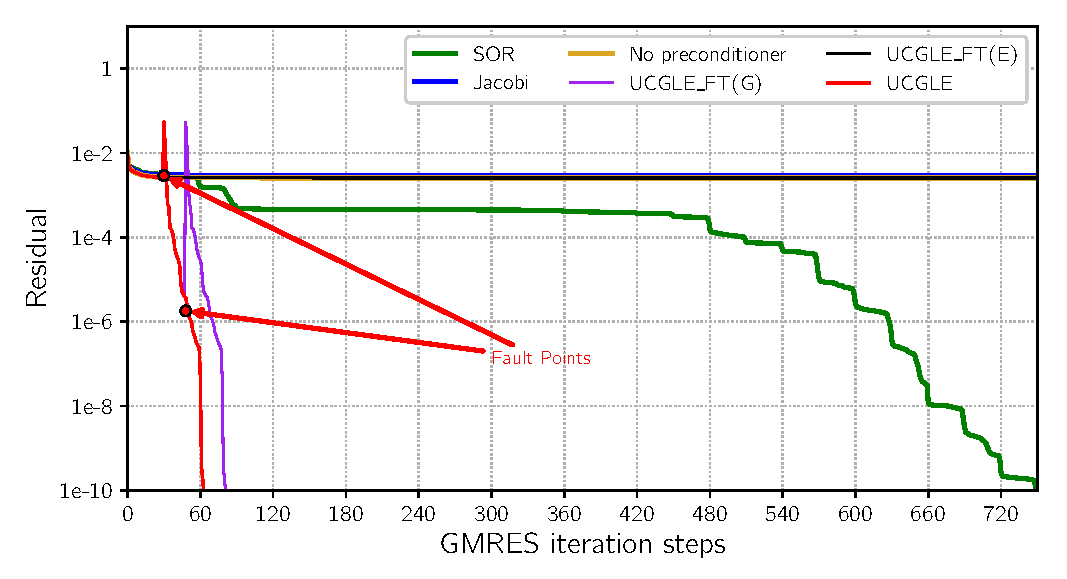
\includegraphics[width=6.2in]{fig/convergence4.eps}
	\caption{$MEG4$: convergence comparison of UCGLE method vs conventional GMRES}
	\label{fig:conv4}
\end{figure}

\begin{table*}[htbp]
	\footnotesize
	\renewcommand{\arraystretch}{1.2}
	\caption{Summary of iteration number for convergence of $4$ test matrices using SOR, Jacobi, non preconditioned GMRES,UCGLE\_FT(G),UCGLE\_FT(G) and UCGLE: red $\times$ in the table presents this solving procedure cannot converge to accurate solution (here absolute residual tolerance \num[round-precision=2,round-mode=figures]{0.0000000001} for GMRES convergence test) in acceptable iteration number ($20000$ here).}
	\label{iterations}
	\centering
	\begin{tabular}{*{7}{c}}
		\toprule
		Matrix Name& SOR & Jacobi & No preconditioner & UCGLE\_FT(G) &UCGLE\_FT(G) & UCGLE \\
		\midrule
		$MEG1$  & 1430 & \textcolor{red}{$\times$} & 1924 & 995 & 1073 & \cellcolor{yellow}900\\
		
		$MEG2$  & 2481 & 3579 & 3027 & 2048 & 2005 & \cellcolor{yellow}1646\\
		
		$MEG3$ & 217 & 386 & 400 & 81 & 347 & \cellcolor{yellow}74\\
		
		$MEG4$ & 750 & \textcolor{red}{$\times$} & \textcolor{red}{$\times$} & 82 & \textcolor{red}{$\times$} & \cellcolor{yellow}64\\
		\bottomrule
	\end{tabular}
\end{table*}

\subsection{Scalability Evaluation}

\textcolor{red}{This section should be rewritten to compare the scaling perfomance both on Tianhe-2 and Romeo. }

For the resolution of large-scale linear systems on the modern supercomputing platforms, the main concern of the conventional preconditioned Krylov methods is the cost of the global communication and synchronization
overheads. We select the test matrix $MEG2$ for the scalability evaluation. The average time cost per iteration of these methods is computed by a fixed number of iterations. Time per iteration is suitable for demonstrating scaling behavior.

\begin{figure}[t]
	\centering
	\begin{tabular}{cc}
		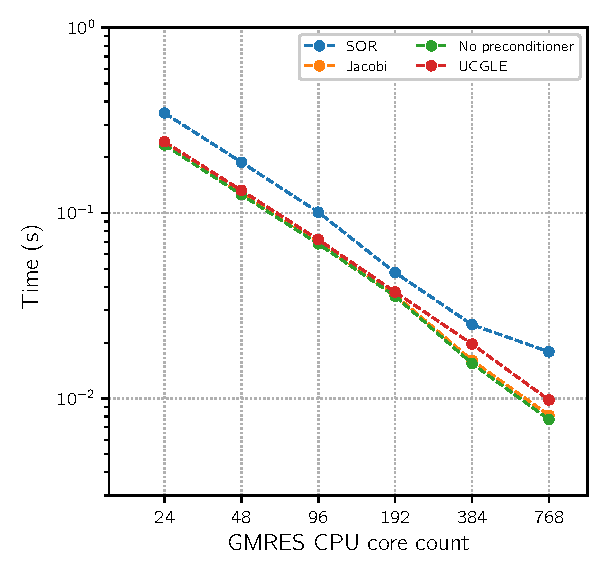
\includegraphics[width=.48\linewidth]{fig/scalable.eps}
		&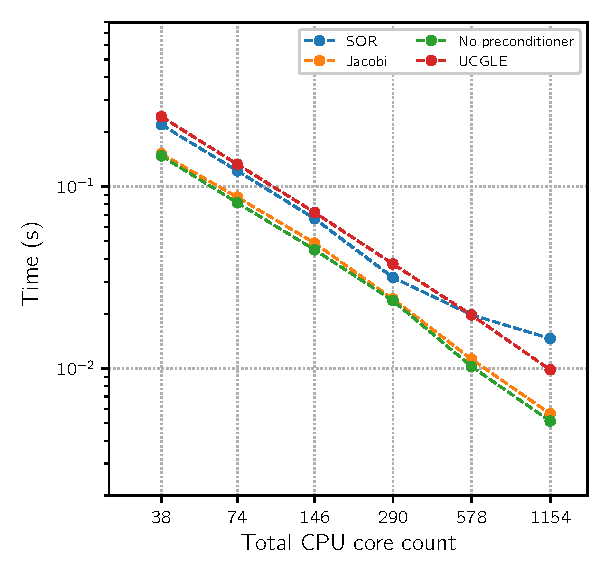
\includegraphics[width=.48\linewidth]{fig/scalable_complet.eps} \\[\abovecaptionskip]
		\small (a)& (b) 
	\end{tabular}
	\caption{Scalability per iteration comparison of UCGLE with GMRES with or without preconditioners on Tianhe-2.}\label{fig:myfig}
\end{figure}

\begin{figure}[t]
	\centering
	\begin{tabular}{cc}
		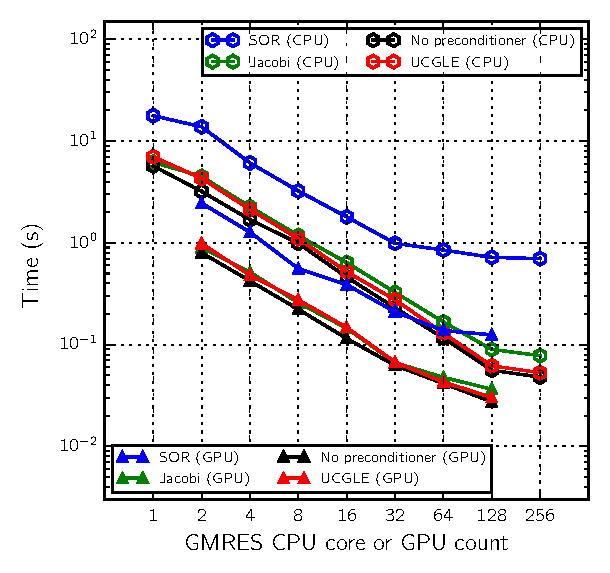
\includegraphics[width=.48\linewidth]{fig/scalable_romeo.eps}
		&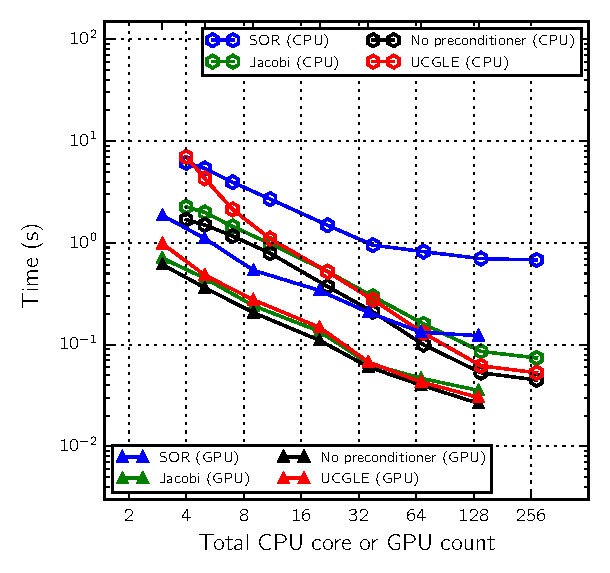
\includegraphics[width=.48\linewidth]{fig/scalable_complet_romeo.eps} \\[\abovecaptionskip]
		\small (a)& (b) 
	\end{tabular}
	\caption{Scalability per iteration comparison of UCGLE with GMRES with or without preconditioners on ROMEO.}\label{fig:myfig2}
\end{figure}

For the evaluation of UCGLE on the homogeneous cluster, the core number of GMRES Component is set respectively to be 24, 48, 96, 192, 384, 768, and both the core number of LS Component and Manager Component is 1. ERAM Component should ensure to supply the approximated eigenvalues in time for each time restart of GMRES Component. Thus we select the core number is respectively 16, 32, 64, 128, 256, 512 referring to different GMRES Component core number. The GMRES core number of conventional GMRES is equal to the one of GMRES Component in UCGLE.

In Fig. \ref{fig:myfig} (a), we can find that these methods have good scalability with the augmentation of computing units except the SOR preconditioned GMRES. The classic GMRES has the smallest time cost per iteration. The Jacobi preconditioner is the simplest preconditioning form for GMRES, and its time cost per iteration is similar to the classic GMRES. The GMRES with SOR preconditioner has the largest time cost per iteration since SOR preconditioned GMRES has the additional matrix-vector and matrix-matrix multiplication operations in each step of the iteration. These operations have global communication and synchronization points. The communication overhead makes the SOR preconditioned GMRES more easily lose its good scalability with the augmentation of computing unit number. There is not much difference between the time cost per iteration of classic GMRES and UCGLE with the help of the asynchronous communication implementation of UCGLE method. Since the resolving part and preconditioning part of UCGLE work independently, its global communication and synchronize points is similar to the classic GMRES without preconditioning. That is the benefits UCGLE's asynchronous communication. 

Since UCGLE requires additional computing units for the master, LS Component and especially ERAM Component, it is necessary to compare UCGLE with other methods when the total computing resource number of UCGLE and other methods keeps the same. Thus we test also the matrix $MEG2$ using conventional methods with the computing unit number to be 38, 74, 146, 290, 578, 1154. The performance comparison is given in Fig. \ref{fig:myfig} (b). We can find that if the computing resource number is small, the time per iteration of classic and conventional preconditioned GMRES is much better than UCGLE since the latter allocates extra computing resources for other components. With the augmentation of computing resources, the scalability of the SOR preconditioned GMRES trends to be bad, and the average time cost per iteration of UCGLE method tends to be better than the SOR preconditioned GMRES with good scalability. Although the scalability of classic and Jacobi is good, and their time per iteration is smaller than UCGLE, but since UCGLE can accelerate the convergence of solving linear systems, thus better performance can be expected.


\subsection{Fault Tolerance Evaluation}

The fault tolerance of UCGLE is studied by the simulation of the loss of either GMRES or ERAM Components. UCGLE\_FT(G) in Fig. \ref{fig:conv1}, Fig. \ref{fig:conv2}, Fig. \ref{fig:conv3} and Fig. \ref{fig:conv4} represents the fault tolerance simulation of GMRES, and UCGLE\_FT(E) implies the fault tolerance simulation of ERAM. 

The failure of ERAM Component is simulated by fixing the execution loop number of ERAM algorithm, in this case, ERAM exits after a fixed number of solving procedures. We mark the ERAM fault points of the two test matrices in Fig. \ref{fig:conv1}, Fig. \ref{fig:conv2},  Fig. \ref{fig:conv3} and Fig. \ref{fig:conv4} : respectively $500$, $560$, $60$ and $30$ iteration step for each case. The UCGLE\_FT(E) curves of the experimentations show that GMRES Component will continue to resolve the systems without LS acceleration. Table \ref{iterations} shows that the iteration number for convergence of UCGLE\_FT(E) is greater than the normal UCGLE method but less than the GMRES method without preconditioning.

The failure of GMRES Component is simulated by setting the allowed iteration number of GMRES algorithm to be much smaller than the needed iteration number for convergence. The values of these cases are respectively $600$, $700$, $70$ and $48$. They are also marked in Fig. \ref{fig:conv1}, Fig. \ref{fig:conv2}, Fig. \ref{fig:conv3} and Fig. \ref{fig:conv4}. We can find that after the quitting of GMRES Component without the finish of its task, ERAM computing units will automatically take over the jobs of GMRES component. The new GMRES resolving procedure will use the temporary solution $x_m$ as a new restarted initial vector received asynchronously from the previous restart procedure of GMRES Component before its failure. In this case, ERAM Component no longer exists. Thus the resolving task can be continued as the classic GMRES without LS preconditioning. In  Fig. \ref{fig:conv1}, Fig. \ref{fig:conv2}, Fig. \ref{fig:conv3} and Fig. \ref{fig:conv4}, we can find the difference between UCGLE\_FT(E) and UCGLE\_FT(G). In UCGLE\_FT(G), the new GMRES Component takes $x_m$ of previous restart procedure. Thus it will repeat the iteration steps of previous restart iterations until the failure of GMRES. Another fact of UCGLE\_FT(G) which cannot be concluded, but can be easily obtained, is that the resolving time will be different if the computing unit numbers of previous GMRES and ERAM Components are different.


\section{Conclusion}

\clearemptydoublepage